\documentclass[conference]{IEEEtran}
\IEEEoverridecommandlockouts

\usepackage{algorithm}
\usepackage{algorithmic}
\usepackage{float}

% ==== Essential Mathematical and Scientific Packages ====
% Package for mathematical symbols, equations, and AMS-specific features
\usepackage{amsmath,amssymb,amsfonts}
% Package for writing algorithms in pseudo-code
\usepackage{algorithmic}
% Package for including and manipulating graphics/images
\usepackage{graphicx}
% Package for special text symbols like degree signs, currency symbols
\usepackage{textcomp}
% Package for colored text and background
\usepackage{xcolor}
% Package for creating subfigures with individual captions
\usepackage{subcaption}
% Package for professional-looking tables with booktabs rules
\usepackage{booktabs}
% Package for typesetting SI units and numbers consistently
\usepackage{siunitx}

% ==== Bibliography Setup (biblatex with Harvard style) ====
% Configure biblatex with specific settings:
% - style=authoryear: Harvard-like citation style
% - backend=biber: Use biber backend instead of traditional BibTeX
% - dashed=false: Don't use dashes for repeated authors
% - maxnames=999: Show all author names (no "et al." truncation)
% - maxcitenames=3: Show up to 3 authors in citations
% - giveninits=true: Use initials for given names
% - urldate=long: Full date format for URL access dates
% - uniquename=false: Don't disambiguate similar author names
% - uniquelist=false: Don't disambiguate similar author lists
\usepackage[style=authoryear, backend=biber, dashed=false, maxnames=999, maxcitenames=3, 
    giveninits=true, urldate=long, uniquename=false, uniquelist=false]{biblatex}

% Specify the bibliography database file
\addbibresource{references.bib}

% ==== Citation Format Customization ====
% Add a comma between author name and year in citations
\renewcommand*{\nameyeardelim}{\addcomma\space}

% ==== Bibliography Entry Format Customization ====
% Remove quotes from titles for various entry types
\DeclareFieldFormat[article,inbook,incollection,inproceedings,patent,thesis,unpublished]{title}{#1}
% Make journal titles italic
\DeclareFieldFormat{journaltitle}{\emph{#1}}

% Format online resources according to Harvard style
\DeclareFieldFormat[online]{title}{\emph{#1}}
\DeclareFieldFormat{url}{Available from: \url{#1}}
\DeclareFieldFormat{urldate}{[Accessed #1]}

% Custom driver for online entries
\DeclareBibliographyDriver{online}{%
  \usebibmacro{bibindex}%
  \usebibmacro{begentry}%
  \usebibmacro{author/editor}%
  \setunit{\labelnamepunct}\newblock
  \usebibmacro{date}%
  \setunit{\addspace}\newblock
  \usebibmacro{title}%
  \newunit\newblock
  \printfield{url}%
  \setunit{\addspace}\newblock
  \printurldate
  \usebibmacro{finentry}%
}

% ==== Journal Entry Format Customization ====
% Customize how journal entries are formatted:
% - Includes journal name
% - Handles series information
% - Formats volume, number, and issue information
\renewbibmacro*{journal+issuetitle}{%
  % Print the journal name
  \usebibmacro{journal}%
  % Handle optional series information
  \iffieldundef{series}
    {}
    {\newunit
     \printfield{series}}%
  % Add volume, number, and electronic ID
  \usebibmacro{volume+number+eid}%
  % Add comma and space before date
  \setunit{\addcomma\space}%
  % Add issue and date information
  \usebibmacro{issue+date}%
  % Add colon and space before issue number
  \setunit{\addcolon\space}%
  % Print the issue
  \usebibmacro{issue}%
  % Prepare for next unit
  \newunit}

% ==== Author Name Format Customization ====
% Define how author names should be formatted:
% - Family name first
% - Given name as initials
% - Handle prefixes (von, van, etc.) and suffixes (Jr., III, etc.)
\DeclareNameFormat{sortname}{%
  \nameparts{#1}%
  \usebibmacro{name:family-given}
    {\namepartfamily}
    {\namepartgiveni}
    {\namepartprefix}
    {\namepartsuffix}%
}
% Apply this format as the default for all names
\DeclareNameAlias{default}{sortname}

% ==== Name List Format Customization ====
% Define how multiple author names are separated
% Add comma and space between multiple names
\DeclareDelimFormat{multinamedelim}{\addcomma\space}
% Use the same delimiter for the final name in the list
\DeclareDelimAlias{finalnamedelim}{multinamedelim}

% ==== Bibliography Printing Command ====
% Define a custom command to print bibliography with optional parameters
% #1 allows passing additional options to \printbibliography
\newcommand{\printbibsection}[1][]{\printbibliography[title=References,#1]} 

\begin{document}

\title{Deep Learning Methods for ArUco Marker Detection and Classification Under Challenging Distortions}

\author{
\IEEEauthorblockN{
    Filip Hanuš\IEEEauthorrefmark{1},
}
\IEEEauthorblockA{
    \IEEEauthorrefmark{1}School of Engineering, College of Art, Technology and Environment,\\
    University of the West of England, Bristol, UK\\
    Email: filip2.hanus@uwe.ac.uk}
}

\maketitle
\begin{abstract}

Blabla

\end{abstract}

\begin{IEEEkeywords}
ArUco Markers, Deep Learning, Computer Vision, Object Detection, Image Classification, Fiducial Markers
\end{IEEEkeywords}

\section{Introduction}

ArUco markers (figure \ref{fig:aruco_marker_basic}) are square visual codes designed for easy detection and identification by computer vision algorithms. 
They are used for positioning, tracking, and navigation in various applications such as robotics, virtual reality, or industrial automation.

\begin{figure}[h]
    \centering
    
\includegraphics[width=0.1\textwidth]{images/aruco-marker-1.png}
    \caption{Basic ArUco marker example}
    \label{fig:aruco_marker_basic}
\end{figure}

Some specific examples of ArUco marker usage can be seen in Figure \ref{fig:aruco_markers}. For their use in these applications, 
they need to be tracked and/or recognised, which creates the need for robust detection and classification methods.

\begin{figure}[h]
    \centering
    \begin{subfigure}[b]{0.45\textwidth}
        \centering
        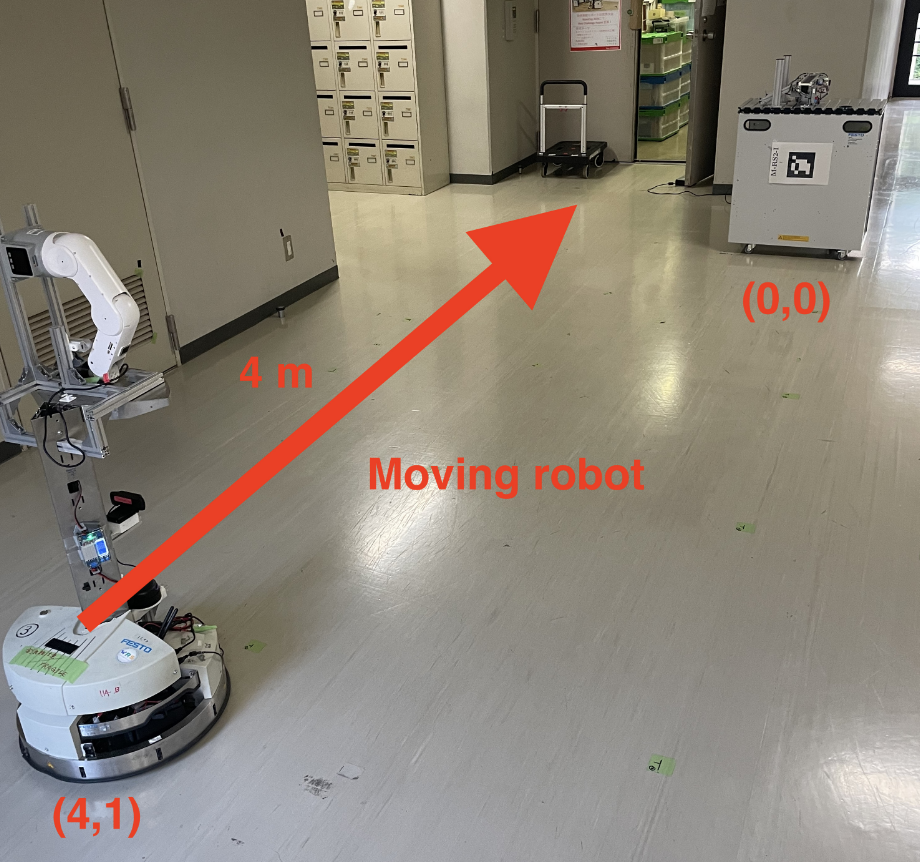
\includegraphics[width=\textwidth]{images/aruco-example-1.png}
        \caption{Robot localisation (\cite{AI-Assisted-Drone-Localization})}
        \label{fig:aruco1}
    \end{subfigure}
    \hfill
    \begin{subfigure}[b]{0.45\textwidth}
        \centering
        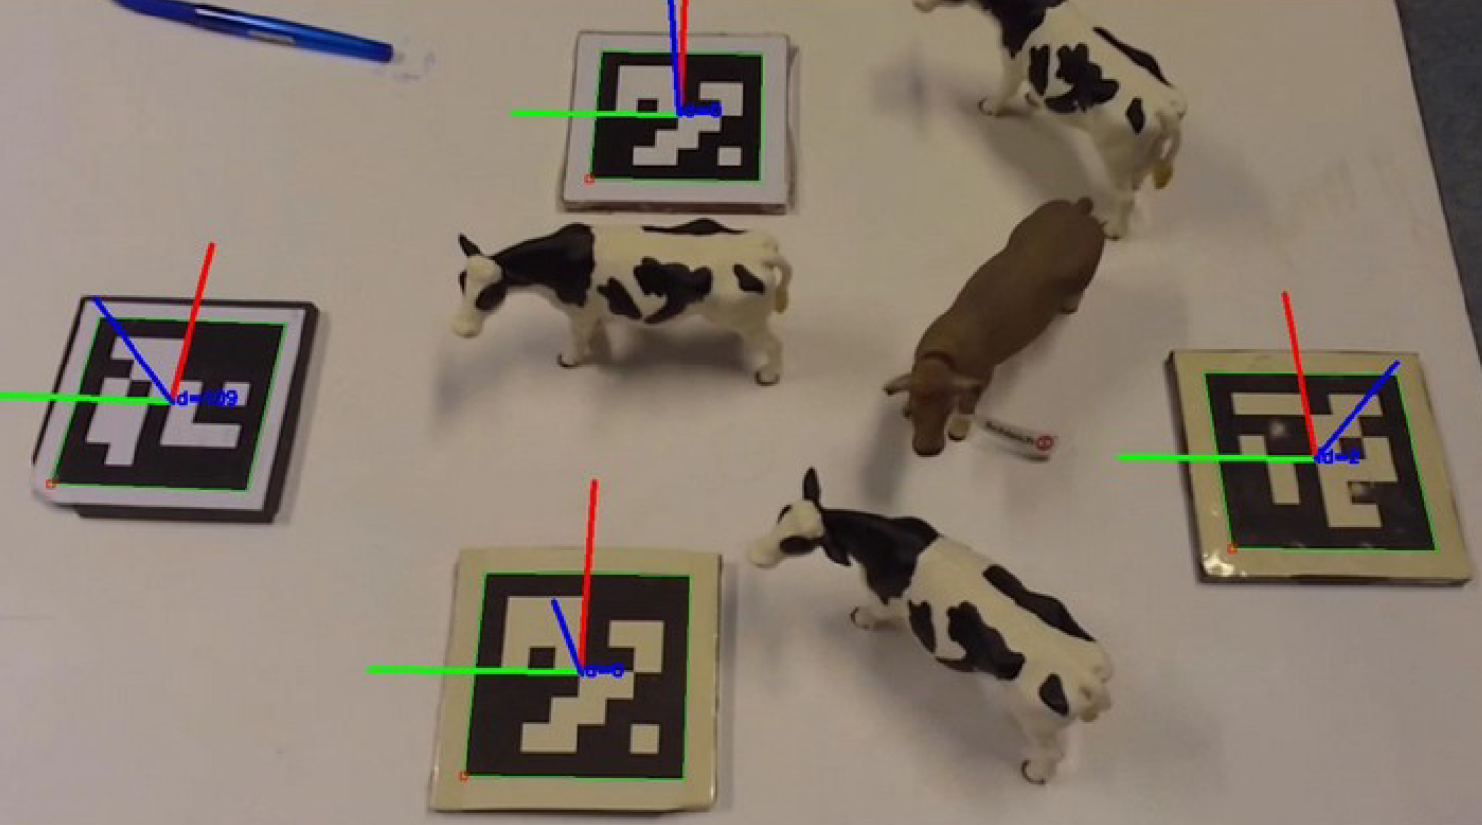
\includegraphics[width=\textwidth]{images/aruco-example-2.png}
        \caption{Drone localisation (\cite{Nakajima2024AboutAE})}
        \label{fig:aruco2}
    \end{subfigure}
    \caption{Examples of ArUco markers in different conditions}
    \label{fig:aruco_markers}
\end{figure}

As \textcite{FiducialMarkerNoisy}, \textcite{ROMERORAMIREZ2021104094}, and others point out, traditional detection methods perform well under controlled 
conditions, but less reliably with real-world challenges, such as rotations, blur and noise. Building on that, this work explores deep learning 
approaches to enhance both detection and classification of ArUco markers under varying conditions. 

This project solves the following challenges:

\begin{enumerate}
  \item Classification of slightly and strongly blurred, noisy and/or rotated ArUco markers,
  \item Detection of slightly and strongly blurred, noisy or rotated ArUco markers in office photos
\end{enumerate}

\section{Classification}

\subsection{Classification Method}

The classification problem was broken down into the following steps:

\begin{enumerate}
  \item Create a data plotter for datasets and results
  \item Develop data augmentation script for prepation of a larger dataset  
  \item Prepare classification network architectures
  \item Design experiment to compare classification architectures and parameters
  \item Train and test the final selected classification model
\end{enumerate}

\subsubsection{Data Preparation}

Firstly, the dataset browser was developed. It allows for easy browsing. It was initially used to browse the dataset and to get an idea of the data. 
The idea was that this same tool would later be used to plot the data and results. This can be seen in Figure \ref{fig:data_browser_1}.

\begin{figure}[h]
  \centering
  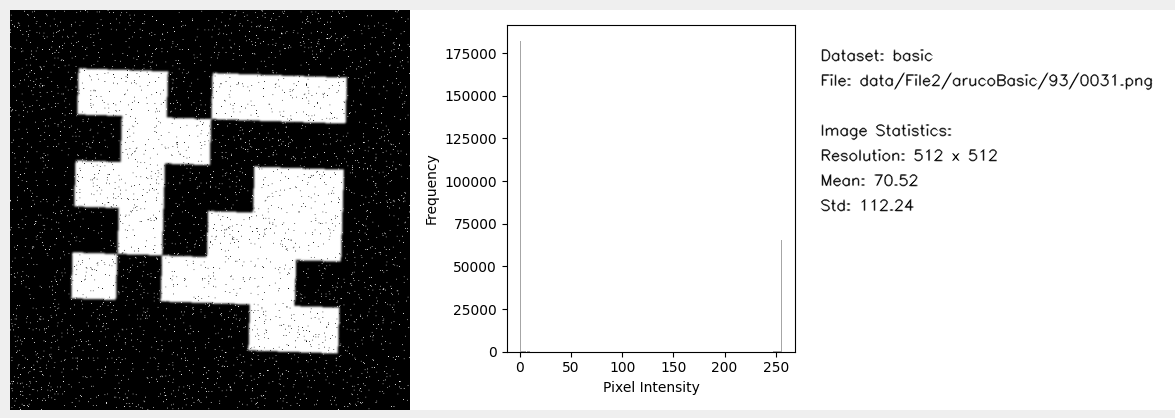
\includegraphics[width=0.5\textwidth]{images/aruco-dataset-browser-1.png}
  \caption{Dataset browser used with the File2 dataset}
  \label{fig:data_browser_1}
\end{figure}

The training pipeline incorporated several data augmentation techniques:

\begin{itemize}
    \item \textbf{Geometric Transformations}:
    \begin{itemize}
        \item Rotations: 0-360° range
        \item Scale variations: 50-100\% of original size
    \end{itemize}
    
    \item \textbf{Image Quality Variations}:
    \begin{itemize}
        \item Gaussian blur ($\sigma$ = 0-14)
        \item Random noise (up to 10\% of pixels)
    \end{itemize}
\end{itemize}


The methodology can be broken down into several key components:

\subsubsection{Network Architectures}

Multiple architectures were evaluated to find the optimal balance between performance and computational efficiency:

\begin{itemize}
    \item \textbf{MinimalCNN}: A lightweight custom architecture with:
    \begin{itemize}
        \item Three convolutional blocks (32$\rightarrow$64$\rightarrow$128 features)
        \item Batch normalization and dropout for regularization
        \item Global average pooling for dimension reduction
    \end{itemize}
    
    \item \textbf{AlexNet Variants}:
    \begin{itemize}
        \item Clean implementation without pre-training
        \item Version with frozen ImageNet pre-trained features
    \end{itemize}
    
    \item \textbf{ResNet18}: Pre-trained on ImageNet with skip connections
    \item \textbf{GoogLeNet}: Pre-trained implementation with inception modules
\end{itemize}

\subsubsection{Training Configuration}

The final training setup was optimized based on experimental results:

\begin{itemize}
    \item \textbf{Optimizer}: Adam with learning rate 3e-4
    \item \textbf{Loss Function}: Cross-entropy
    \item \textbf{Batch Size}: 32 (optimal for memory/performance trade-off)
    \item \textbf{Training Duration}: 50 epochs with early stopping
    \item \textbf{Data Split}: 95\% training, 2.5\% validation, 2.5\% test
\end{itemize}

\subsubsection{Key Design Decisions}

The implementation followed this algorithmic workflow:

\begin{figure}[H]
\begin{algorithm}[H]
\caption{ArUco Classification Training Pipeline}
\begin{algorithmic}[1]
\STATE Load pre-trained model (GoogLeNet)
\STATE Apply data augmentation transforms
\FOR{each epoch in training}
    \STATE Forward pass through network
    \STATE Calculate cross-entropy loss
    \STATE Backpropagate and update weights
    \IF{validation accuracy > 99.9\%}
        \STATE Early stopping
    \ENDIF
\ENDFOR
\STATE Evaluate on File2 (basic) and File3 (challenging)
\end{algorithmic}
\end{algorithm}
\caption{Classification training workflow}
\end{figure}

\subsection{Results: Classification}

Presentation of experimental setup

Datasets used (Files 2, 3, and custom datasets)
Evaluation metrics (accuracy, precision, recall, F1-score)

Numerical results and analysis

Comparison across different network architectures
Effect of parameters (learning rate, batch size, number of training images)
Graphs illustrating training accuracy, confusion matrices

Discussion of performance trends

Strengths and weaknesses observed
Cases of misclassification and potential causes

\section{Detection}

The detection problem was broken down into the following steps:

\begin{enumerate}
  \item Adapt and prepare the data plotter for detection datasets and results
  \item Develop data augmentation script
  \item Prepare detection network architectures
  \item Design experiment to compare detection architectures and settings
  \item Train and test the final detection model
\end{enumerate}


\begin{figure}[h]
  \centering
  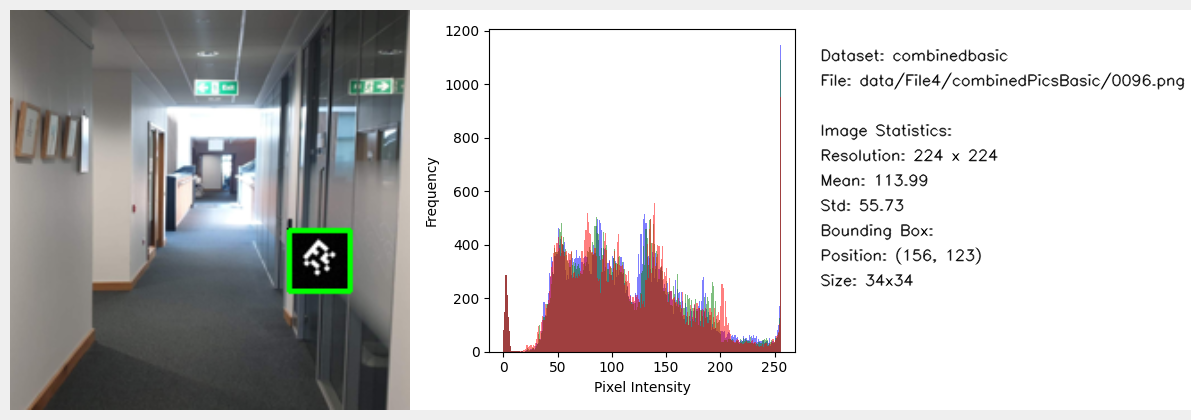
\includegraphics[width=0.5\textwidth]{images/aruco-dataset-browser-2.png}
  \caption{Dataset browser used with the File4 dataset}
  \label{fig:data_browser_2}
\end{figure}


\subsection{Method: Detection}

Overview of detection approach

Data preparation: merging ArUco markers with office images
Selection of detection models (e.g., RetinaNet-ResNet50, FasterRCNN-ResNet50, MobileNetV3-Large-FPN)
Training configuration and hyperparameters

Algorithmic workflow (with diagrams/pseudocode)

Preprocessing and annotation generation
Model training loop for detection
Post-processing steps (bounding box adjustments, non-max suppression)

Challenges and considerations

Handling strong distortions and occlusions
GPU memory management and batch size limitations

\subsection{Results: Detection}

Presentation of experimental setup

Datasets used (Files 4, 5, and custom datasets)
Evaluation metrics (Mean IoU, MAE, detection success rates)

Numerical results and analysis

Performance comparison of different detection architectures
Impact of distortions on detection accuracy
Visualisation of detection outputs and failure cases

Discussion on detection performance

Analysis of false negatives/positives
Critical factors affecting detection success

\section{Conclusion}

Summary of methodologies and key findings in classification and detection
Critical analysis of strengths and weaknesses of approaches
Insights into factors affecting performance
Suggestions for improvements and areas for future research

Further dataset expansion (synthetic or real-world captures)
Refinement of network architectures and training strategies
Enhanced evaluation techniques and theoretical analysis

\printbibsection

\appendices

\renewcommand{\thesection}{\Alph{section}}

\section{Detailed Network Architecture}

Appendix 1

\section{Classification Network}

Appendix 2

\end{document}
